\clearpage
\section{Visual Detection and Grid Mapping}
The detector, model metrics, and grid processing in this section apply to the physical experiment. The recorded simulation uses HSV color segmentation instead, as described in Section~\ref{sec:simulation}.

\label{sec:vision}

\subsection{Six-class detection and training method}

The vision system answers two questions before the robot moves: what kind of object is present, and which pickup cell contains it? We used YOLO11 to predict a class, a bounding box, and a confidence score for each object. The six labels were \file{blue_cube}, \file{green_cube}, \file{pink_cube}, \file{yellow_cube}, \file{red_cuboid}, and \file{orange_bridge}. The detector kept these labels for inspection, while the task controller reduced them to two sorting groups. The four cube classes went to the right area. The red cuboid and orange bridge went to the left area. In this project, ``v4'' means the fourth project model version, not the YOLOv4 network.\src{defense,vision}

The defense slides describe training with a $640\times640$ input, the AdamW optimizer, light data augmentation, and 35 epochs. Each training object had a class label and a box. The positive samples covered different colors, shapes, and views. We also included difficult background samples, such as an empty desk, cables, and the robot body. These negative samples helped the detector learn when it should produce no object box. This was useful because a background error could otherwise create a false pickup request.\src{defense}

The training, validation, and test sets had different roles. Training changed the model weights; validation helped select the saved weights; the test set checked detection quality after training. The selected model was then used for CUDA inference on the Jetson. Model evaluation results are given in Section 8.\src{defense}

Data quality was as important as the training settings. Boxes need to cover the object consistently, and labels need special care for red/pink views, touching objects, and partial occlusion. Background images should resemble the actual work area. Video frames close in time can be very similar, so a test on separately recorded scenes gives stronger evidence of general use than a random split of nearby frames. The supplied earlier data-building script uses time blocks for splitting; the final v4 dataset size is not stated here because a matching final dataset summary was not supplied.\src{vision}

\begin{figure}[H]
    \centering
    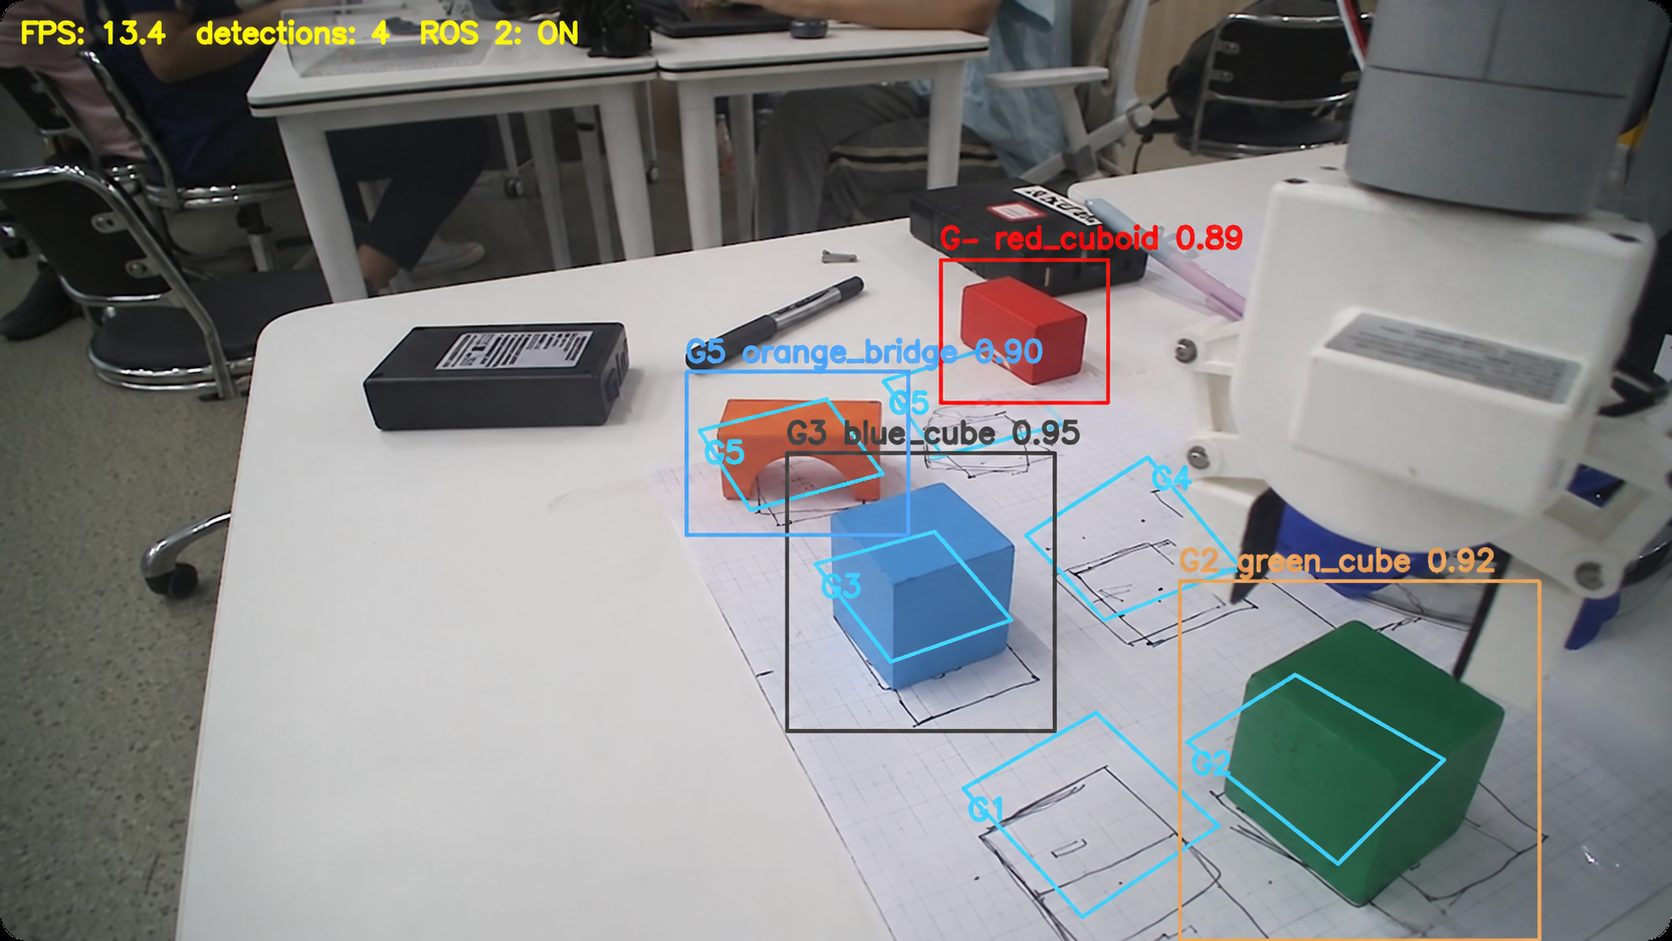
\includegraphics[width=0.92\textwidth]{figures/vision_scene.png}
    \caption{Detection and grid overlays in the experimental scene, reproduced from defense slide 4. Boxes show class names and confidence scores; blue polygons mark pickup regions. The displayed 13.4 FPS is one snapshot value, not a measured average over a complete run.\src{defense}}
    \label{fig:vision-scene}
\end{figure}

\Needspace{8\baselineskip}
\subsection{A second check for red and pink objects}

The red cuboid and pink cube were a difficult pair. Their colors could look similar under the camera, and a cuboid viewed from one end could appear nearly square. An error between these classes also changed the destination, so it deserved special attention. We therefore used the separate \file{red_pink_shape_classifier_v2.pt} model to check the object crop after the main detection.\src{vision}

For a pink or red detection, the program added padding equal to 8\% of the box width and height on each side. It kept the crop inside the image and passed it to the second model with an input size of 224. The correction rule was one way: an original pink-cube label changed to red cuboid only if the second model predicted red with a score of at least 0.55. An original red label was kept. The box position and main detector confidence were also kept.\src{vision}

The second classifier only processes candidate crops from the main detector, so it cannot recover an object that YOLO misses.

\subsection{Calibrating six image regions}

The table had six fixed pickup cells, named G1 to G6. Each cell was linked to taught robot poses. The camera therefore needed to select the correct cell, rather than calculate a new three-dimensional grasp pose for every object. The calibration program represented each cell by a four-corner polygon in the $1280\times720$ camera image. The operator clicked its corners in the browser view and then tested points inside and outside the regions.\src{calibration}

Before saving, the program checked that all six IDs were present, the corners were distinct and inside the image, and each polygon formed a valid convex quadrilateral. It rejected regions with an area below 1,000 square pixels and overlaps larger than two square pixels. These checks caught incomplete or poorly drawn regions before they reached the controller. The accepted polygons were stored in \file{regions.yaml}.\src{calibration}

The camera and table layout needed to stay fixed after this step. A change in camera position could move a visible cell even though its stored polygon stayed unchanged. Likewise, moving the robot base could break the link between a cell and its taught pose. The empty example configuration was only a template; the real experiment required the measured regions for its own setup.

\subsection{From a detection box to a pickup cell}

Let the top-left and bottom-right corners of a detected box be $(x_1,y_1)$ and $(x_2,y_2)$. Its image center is
\begin{equation}
    \mathbf{c}=(c_x,c_y)
    =\left(\frac{x_1+x_2}{2},\frac{y_1+y_2}{2}\right).
\end{equation}
For region polygon $P_i$, define the set of matching cells as
\begin{equation}
    \mathcal{G}(\mathbf{c})=\{i\in\{1,\ldots,6\}:\mathbf{c}\in P_i\}.
\end{equation}
The program assigns a grid ID only when $|\mathcal{G}(\mathbf{c})|=1$. A center outside all regions has no pickup cell. A center assigned to more than one region is also left unresolved. The controller uses a point-in-polygon calculation for this decision.\src{vision,controller}

Vision selects the cell, and the arm uses its stored approach and grasp poses. Objects need to stay near the taught pickup positions because this method does not estimate depth or adjust the grasp within a cell.

\begin{figure}[H]\centering
\begin{tikzpicture}[font=\small,>=Latex]
\foreach \id/\x/\y in {1/0/1.15,2/1.55/1.15,3/3.1/1.15,4/0/0,5/1.55/0,6/3.1/0}{
\draw[Navy,fill=PaleBlue] (\x,\y) rectangle ++(1.4,1.0);
\node[anchor=north west] at (\x+0.1,\y+0.93) {G\id};}
\draw[Blue,thick] (3.50,1.27) rectangle (4.30,1.77);
\fill[Teal] (3.90,1.52) circle (2.6pt);
\node[draw=Navy,align=center,text width=4.7cm,minimum height=1.5cm] (poses) at (8.3,1.1)
{Grid 3 pose pair\\\texttt{grid\_3\_approach}\\\texttt{grid\_3\_grasp}};
\draw[->,thick,Teal] (4.5,1.52)--(poses.west);
\node[font=\scriptsize] at (5.2,1.95) {cell ID};
\node[align=center,font=\footnotesize] at (2.25,-0.55) {Image region and box center};
\node[align=center,font=\footnotesize] at (8.3,-0.55) {Class group separately selects left or right};
\end{tikzpicture}
\caption{Discrete image-to-pose mapping. Grid 3 is an illustrative example; the drawing is a schematic, not the measured camera calibration.}
\end{figure}

\subsection{Stable decisions across several frames}

A box in one frame was not enough to trigger a pick. For each cell, the controller first converted the current detections into a sorting observation. No box gave \file{EMPTY}; an unsupported class gave \file{UNKNOWN}; and boxes from different sorting groups gave \file{MULTIPLE}. These unresolved cases did not become pickup targets.\src{controller}

The formal ROS controller treated several boxes from the same group as one group observation and used the highest-confidence box as its representative. This addressed cases where one physical cube produced overlapping boxes with different color labels. Since all cube labels shared a destination, those duplicate labels did not need different actions. The method still assumed one physical object per pickup cell: it could not distinguish duplicate boxes from two real objects of the same group.\src{controller}

The controller then stored the last seven observations, $o_{t-6},\ldots,o_t$. For each possible group or state $s$, it counted
\begin{equation}
    N_t(s)=\sum_{k=t-6}^{t}\mathbf{1}[o_k=s].
\end{equation}
After the window was full, a state was stable if it received at least five votes. Stable cube and other observations became \file{READY_CUBE} and \file{READY_OTHER}. Stable \file{EMPTY}, \file{UNKNOWN}, and \file{MULTIPLE} states were kept. If no state received five votes, the cell remained a candidate. Before issuing a request, the controller also required the current group to agree with the stable ready state. Voting was thus based on the sorting group, not an exact color label.\src{controller}

We set the detector confidence threshold to 0.25. Unique center-in-polygon assignment determines the source grid, and the controller requires five matching sorting-group observations in a seven-observation window. These checks suppress brief detection changes before a new target becomes ready.\src{vision,controller}

The confidence threshold, the NMS overlap threshold, and the temporal vote solve different problems. Confidence controls which candidate boxes are kept. NMS, configured with an IoU threshold of 0.45, reduces overlapping detections. The vote compares observations across frames. A lower confidence threshold can retain weak targets but also retain more false boxes. Persistent false detections can still pass these checks.
